\documentclass[../../main.tex]{subfiles}

\begin{document}
\problem{52}
\begin{wts}
How many HTTP GET requests are sent by your web browser? 
\end{wts}
\begin{proof}
Consider the following,\\
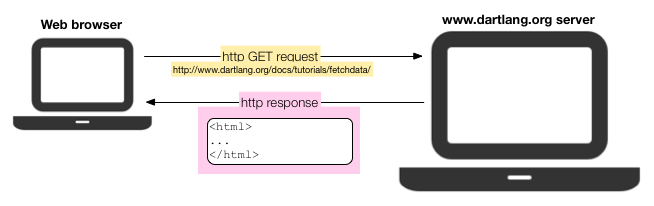
\includegraphics[width=\textwidth]{subfiles/images/L5_Manual/L5N2_ DNS & HTTP_PAGE21_12_Image137.png}
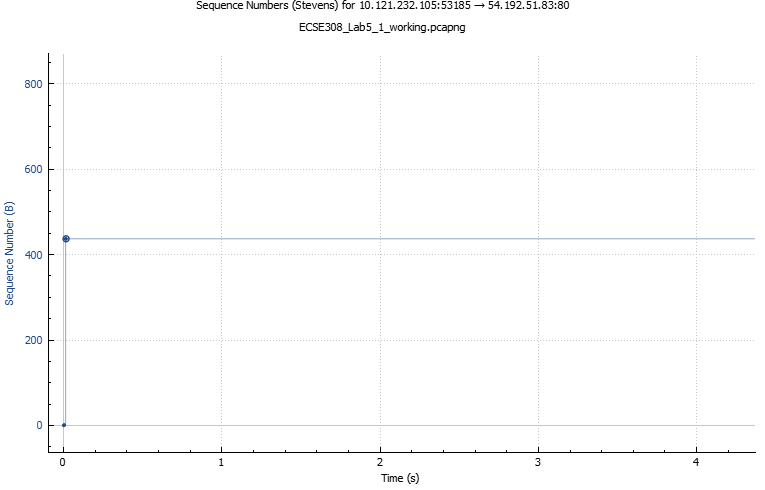
\includegraphics[width=\textwidth]{subfiles/images/ECSE_308_Lab_5_1_SUPA_PAGE5_18_Image53.png}
On an abstract level, an application process that resides on the host’s computer dedicates a buffer region in a transmit control block (TCB). The size the TCB is finite, so the sender must be aware of the remaining available buffer space left in the TCB. For the simple case where the application process reads the data immediately, in technical terms we say that the right window edge advances with the left — the ‘window’ field advertises the difference between the last byte sent and the last byte ACKed by the destination TCP.\\

    If we relax the assumption that the destination application process does not read the incoming byte stream immediately, then a fast sender who sends multiple TCP segments within a short period of time may receive an acknowledge packet of the form
    
    \[\code{ACK XXXX, WIN 0}\]
    
    Telling the sender to stop sending segments, even though all packets are acknowledged, the destination process has yet to read them (and thus remove them from the TCB). Numerous simplifications have been made in the previous heuristic explanation and the reader is encouraged to read the RFCs for a complete introduction.
\subfile{./Folland/Theorem6_15.tex}
\newcommand{\pxf}{P_{\mathbf{X}}(f)}
\newcommand{\pyf}{P_{\mathbf{y}}(f)}
\newcommand{\hf}{\mathbf{H}(f)}
\newcommand{\xf}{\mathbf{X}(f)}
\newcommand{\yf}{\mathbf{Y}(f)}
\subsection*{B5 ISI and AWGN}
\begin{wtr}
\begin{enumerate}
    \item[]
    \item Nyquist Criterion for Digital Modulation.
    \[
    \varepsilon=\dfrac{f_s}{B}\leq 1
    \]
    Where $f_s$ is the symbol rate transmitted over a passband bandwidth $B$, without ISI.
    \item Shannon's Theorem for AWGN bitrate
    \[
    \varepsilon_{max} = \log_2(1+SNR)
    \]
    \item Effective bitrate $R_b$ (bits per sec),
    \[
    R_b = f_s\log_2|\cal{A}|,\quad |\cal{A}| \text{ size of alphabet}
    \]
\end{enumerate}
    
\end{wtr}
\end{proof}

\end{document}